\chapter{Borel's Conjecture}\label{c1}

We\pageoriginale start these lectures by defining a concept central to
this course.
\begin{defi}\label{c1:defi1.1}
  A topological space is called aspherical if $\pi_n(X)=0$ for $n \neq
  1$. Here $\pi_n(X)$ denotes the $n^{\text{th}}$ homotopy group of $X$.
\end{defi}

If we assume $X$ to be a CW-complex, then the above definition is
equivalent to saying that the universal cover of $X$ is contractible.

Let us recall a well-known result due to Hurewicz and then sketch its
proof. 

\begin{thm}\label{c1:thm1.2}
  Let $X$ and $Y$ be aspherical CW-complexes and 
$$
\alpha : \pi_1 (X)
  \to \pi_1 (Y)
$$ 
be an isomorphism. Then $\alpha$ is induced by a
  homotopy equivalence $f: X \to Y$.
\end{thm}

\begin{proof}
  We may assume (after some fuss) that the 1-skeleton of $X$, denoted
  by $X^1$, is a wedge of circles. Hence we get a map $f^1 : X^1 \to
  Y$ by sending the $i$-th circle, $a_i$ in $X^1$ to a loop in $Y$
  representing $\alpha ([a_i])$ where $[a_i]$ is the homotopy class of
  $a_i$. This map extends over the 2-skeleton $X^2$ since the boundary
  of any 2-cell in $X$ (thought of as an element in $\pi_1 (S^1)$)
  maps to the trivial element of $\pi_1 (Y)$ via $(f^1)_*$. We then
  easily extend the map mover all of $X$ by using the fact that $Y$ is
  aspherical. Thus $f$ is constructed satisfying $f_* =\alpha$. This
  map is clearly a weak homotopy equivalence since both $X$ and $Y$
  are aspherical. And it is therefore a homotopy equivalence since
  both $X$ and $Y$ are CW-complexes.
\end{proof}

In view of the above theorem, one might ask whether any two aspherical
CW-complexes with isomorphic fundamental groups are homeomorphic. The
following examples show that this is not true.

\begin{figure}[H]
  \centering{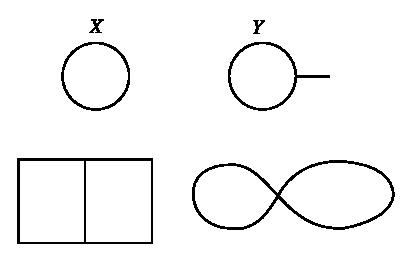
\includegraphics{vol86-figures/fig1.eps}}
\end{figure}

It\pageoriginale is clear these examples that one should require $X$ and $Y$ to have
a fixed local homeomorphism type. But the answer to the above question
is still no, even if we assume that the aspherical CW-complexes with
isomorphic fundamental groups are alos manifolds of the same
dimension. A conuterexample in this case is 
\begin{center}
  $X= S^1 \times \mathbb{R}$ and $Y=$ M\"obius band.
\end{center}

But the following conjecture made by Borel about 1955 is still open.

\begin{conj}[Borel]\label{c1:conj1.3}
  If $M$ and $N$ are closed aspherical manifolds with isomorphic
  fundamental groups, then they are homeomorphic; in fact, the
  homeomorphism can be chosen to induce the given isomorphism.
\end{conj}

\begin{remark*}
  The following strengthenings of Borel's conjecture are both false as
  the next examples show.
  \begin{enumerate}[(i)]
    \item All closed aspherical manifolds support a smooth structure.
      \item Any two closed smooth aspherical manifolds with isomorphic
        fundamental groups are diffeomorphic.
  \end{enumerate}
\end{remark*}

Let $T^n$ denote the $n$-dimensional torus; i.e., $T^n = S^1 \times
S^1 \times \ldots \times S^1$ ($n$-factors) where $S^1$ is the
circle. Browder \cite{13} constructed a smooth manifold which is
homeomorphic but not\pageoriginale diffeomorphic to $T^\tau$. This
shows that (ii) is false. In fact, it follows from later results that
$T^n$ and the connected sum $T^n \# \sum^n$ are homeomorphic but not
diffeomorphic if $n \geq 5$ and $\sum^n$ is any exotic
$n$-sphere. That is,  $\sum^n$ is a smooth manifold which is
homeomorphic but not diffeomorphic to the standard $n$-dimensional
sphere $S^n$, cf. \cite{65}. On the other hand, M. Davis and
J.C. Hausmann \cite{23} constructed an example of a closed aspherical
manifold which does not support any differentiable structure proving
(i) to be false as well Moreover, M. Davis and T. Januszkiewcz
\cite{24} gave an example of a closed aspherical manifold which can
not be triangulated.

\setcounter{section}{3}
\section{Examples of Aspherical Manifolds}\label{c1:sec1.4}

\begin{enumerate}[(1)]
\item Any complete non-positively curved Riemannian manifold is
  aspherical. This follows from the Cartan-Hadamard Theorem. Special
  cases are:
  \begin{enumerate}[(i)]
    \item flat Riemannian manifolds,
      \item hyperbolic manifolds,
        \item locally symmetric space of non-compact type.
  \end{enumerate}
  \item If $G$ is a virtually connected Lie group, $k$ a maximal
    compact subgroup, and $\Gamma$ a discrete  torsion free subgroup
    of $G$, then the double coset space $\Gamma\backslash G/K$ is
    aspherical. In this case, $G/K$ is diffeomorphic to $\mathbb{R}^n$
    for some integer $n$. In the special case where $G$ is virtually
    nilpotent and $\pi_1 G=1$, the double coset space
    $\Gamma\backslash G/K$ is called an infranilmanifold.
\end{enumerate}

But there are many other aspherical manifolds which are not of the
types (1) or (2). For example, the closed smooth aspherical manifolds
constructed by Davis \cite{21} are not of these types since their
universal covers are not even homeomorphic to $\mathbb{R}^n$. This is
particularly surprising since the fundamental groups of these
manifolds are relatively ``tame''. In fact, they are finite index
subgroups of certain Coxeter groups. We will discuss his construction
in Lecture 3.

Gromov \cite{54} has more recently constructed many more examples of
aspherical manifolds. Given any closed manifold $N^n$ which is a
polyhedron, he constructed a closed aspherical manifold\pageoriginale
$M^n$ and a degree 1 map $f: M^n \to N^n$. The reason these manifolds
$M^n$ are aspherical is they are nonpositively curved complexes in the
sense of Alexandroff.

\begin{remark*}
  Borel's conjecture implies Poincare's conjecture which says that any
  simply connected closed 3-manifold is homeomorphic to the unit
  sphere $S^3$ in $\mathbb{R}^4$. This is seen as follows.Let $\sum^3$
  be a counterexample to Poincare's conjecture, and consider the
  connected sum $M=T^3 \# \sum^3$, where $T^3$ again denotes $S^1
  \times S^1 \times S^1$. Van Kampen's theorem shows that $T^3$ and
  $M^3$ have isomorphic fundamental groups. And $M$ is seen to be
  aspherical by applying the Hurewicz isomorphism theorem to the
  universal cover of $T^3 \# \sum^3$. Borel's conjecture is
  contradicted by showing that $T^3\# \sum^3$ is not homeomorphic to
  $T^3$. For this we use the following two results.
\end{remark*}

\setcounter{lemma}{4}
\begin{thm}[Schoenflies Theorem]\label{c1:thm1.5}
  Let $f: S^2 \to S^3$ be a bicollared embedding, then $f(S^2)$ bounds
  closed (topological) balls on both sides.
\end{thm}

\begin{thm}[Alexander's Trick]\label{c1:thm1.6}
  Let $h: S^n \to S^n$ be any homeomorphism. Then $h$ extends to a
  homeomorphism $\ob{h}: \mathbb{D}^{n+1} \to \mathbb{D}^{n+1}$, where
  $\mathbb{D}^{n+1}$ denotes the closed ball of radius 1 in
  $\mathbb{R}^{n+1}$ which bounds $S^n$.
\end{thm}

Now if $T^3 \# \sum^3$ were homeomorphic to $T^3$, then the universal
cover of $T^3 \# \sum^3$ is homeomorphic to
$\mathbb{R}^3$. Consequently, the Schoenflies theorem shows that
$\sum^3$-Int $\mathbb{D}^3$ is homeomorphic to $\mathbb{D}^3$. (This
Int $\mathbb{D}^3$ is the interior of the 3-dimensional ball removed
from $\sum^3$ in forming the connected sum with $T^3$.) Now applying
Alexander's trick, we get $\sum^3$ is homeomorphic to $S^3$. It
follows that $T^3\# \sum^3$ is not homeomorphic to $T^3$.
